% Resultados por RQ (S03-08, #127). Valores gerados por `python -m lab03.analysis.*`
% a partir de analysis/base_repositorios.csv; ver Lab-03/analysis/README.md.
\providecommand{\pendente}[1]{\textbf{[Pendente: #1]}}

\section{Resultados}

Os resultados abaixo usam os 300 repositórios do dataset congelado
(\texttt{data/amostra\_completa.json.gz}), achatados em uma linha por
repositório (\texttt{analysis/base\_repositorios.csv}). Seguindo o protocolo,
reportam-se mediana e IQR. Métricas ausentes não são imputadas, e por isso o
$n$ varia por análise. Toda correção para comparações múltiplas usa Holm, com
$\alpha = 0{,}05$.

\subsection{RQ01 a RQ04: métricas DORA}

A Tabela~\ref{tab:rq01-rq04} resume as quatro métricas por repositório. O $n$
válido varia porque 11 repositórios não têm release avaliável para lead time e
CFR (b), e 32 não têm episódio de recuperação encerrado.

\begin{table}[ht]
\centering
\caption{RQ01--RQ04: distribuição por repositório. Fontes:
\texttt{analysis/rq01\_rq02/} e \texttt{analysis/rq03\_rq04/}
(\texttt{lab03.analysis.rq01\_rq02}, \texttt{lab03.analysis.rq03\_rq04}).}
\label{tab:rq01-rq04}
\small
\begin{tabular}{lrrr}
\hline
Métrica & $n$ & Mediana & [Q1--Q3] \\
\hline
Frequência (releases/semana) & 300 & 0,268 & [0,134--0,555] \\
Lead time (a), por release (h) & 289 & 250,8 & [70,3--756,5] \\
Lead time (b), por commit (h) & 289 & 169,4 & [53,9--546,0] \\
CFR (a), runs de CI com falha & 300 & 0,054 & [0,020--0,142] \\
CFR (b), release corretiva em 7 dias & 289 & 0,292 & [0,125--0,522] \\
Recuperação (h) & 268 & 4,89 & [0,84--21,48] \\
\hline
\end{tabular}
\end{table}

\textbf{RQ01.} A mediana é de uma release a cada quatro semanas, e 266 dos 300
repositórios (89\%) publicam menos de uma por semana, o que sustenta a H01.
Nove repositórios não publicaram release na janela.

\textbf{RQ02.} O lead time por release supera o por commit nas medianas (250,8
h contra 169,4 h) e em 212 dos 289 repositórios (73\%), como previa a H02. A
variante (a) dá peso a cada release e cresce quando uma entrega inclui um
commit antigo, enquanto a (b) dilui esse commit entre os demais
(Figura~\ref{fig:rq01-rq02}).

\begin{figure}[ht]
\centering
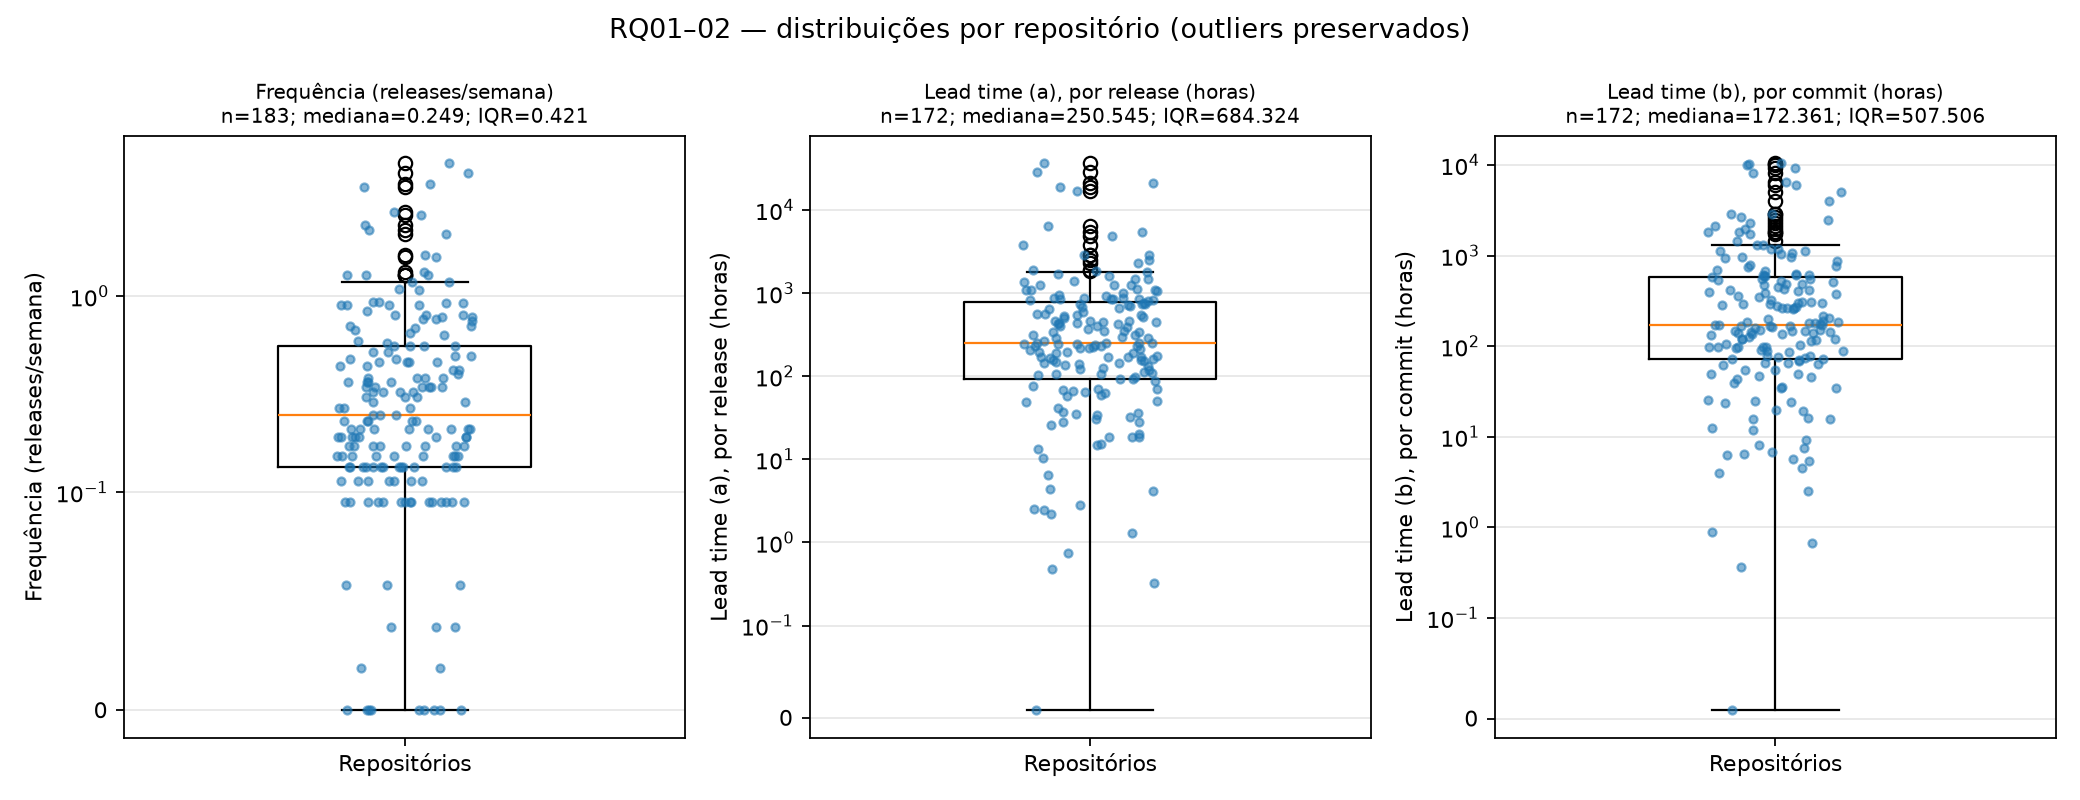
\includegraphics[width=\textwidth]{rq01_rq02/rq01_rq02_distribuicoes.png}
\caption{RQ01--RQ02: distribuições de frequência e lead time (a) e (b), em
escala \textit{symlog}, com todos os outliers preservados.}
\label{fig:rq01-rq02}
\end{figure}

\textbf{RQ03.} As duas variantes de CFR divergem, como previa a H03. Nos 289
repositórios com ambas, a mediana da diferença CFR (b) $-$ CFR (a) é 0,200 (IQR
0,409), com o CFR (b) mais de cinco vezes maior nas medianas
(Figura~\ref{fig:rq03}). Parte dessa distância vem da própria heurística: a
validação parcial (Seção~\ref{sec:validacao-cfrb}) indica que o CFR (b)
superestima as releases corretivas. Nenhuma das duas variantes observa falha em
produção.

\begin{figure}[ht]
\centering
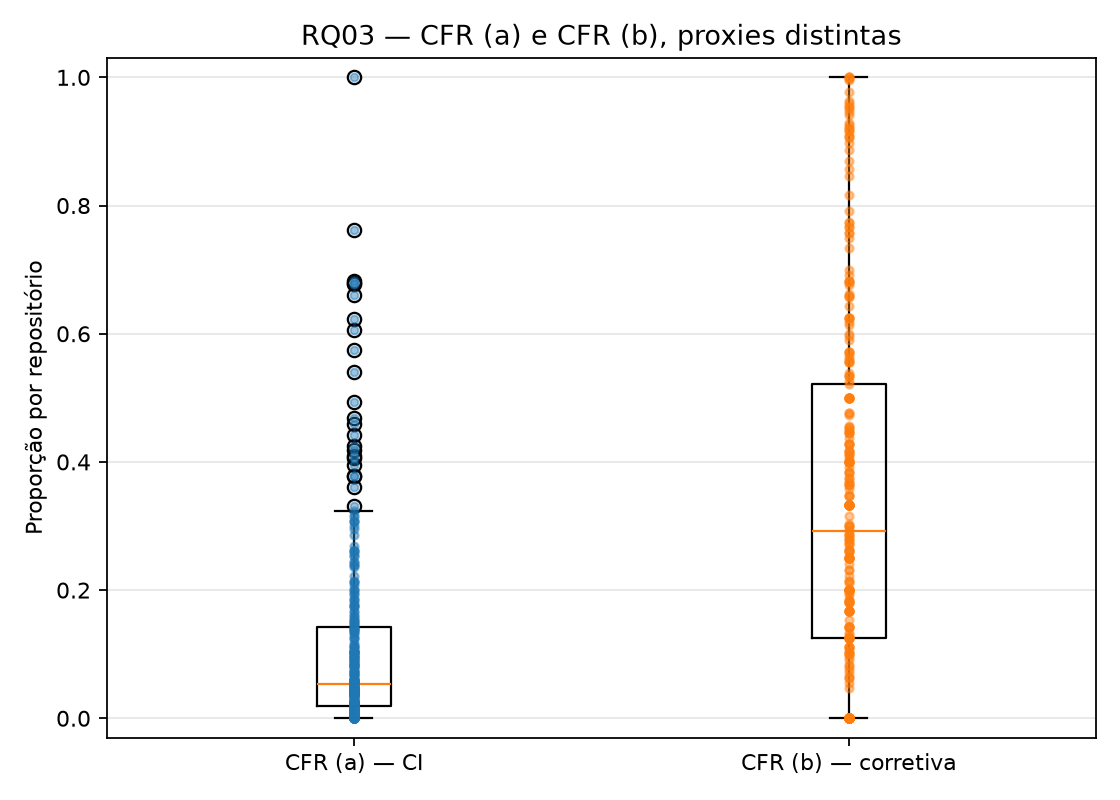
\includegraphics[width=0.7\textwidth]{rq03_rq04/rq03_cfr_comparacao.png}
\caption{RQ03: comparação entre CFR (a) e CFR (b) por repositório.}
\label{fig:rq03}
\end{figure}

\textbf{RQ04.} A recuperação é assimétrica, como previa a H04: mediana de 4,9 h,
com terceiro quartil de 21,5 h. Dos 4.119 episódios, 75 (1,8\%) não foram
encerrados na janela. Eles foram mantidos como censurados, sem tempo imputado.
No CFR (b), 251 das 8.518 releases (2,9\%) são censuradas por não terem os sete
dias seguintes inteiros na janela.

A Tabela~\ref{tab:c1} mostra a classificação DORA de referência (C1), com os
cortes do enunciado. A categoria geral é a mediana das quatro pontuações,
arredondada para baixo, e só é emitida quando as quatro métricas são
observadas. Por isso 40 repositórios ficam sem categoria geral.

\begin{table}[ht]
\centering
\caption{Classificação DORA C1 por métrica e geral (300 repositórios). Fonte:
\texttt{analysis/c1\_reference/c1\_resultados.json}
(\texttt{lab03.analysis.c1\_reference}).}
\label{tab:c1}
\small
\begin{tabular}{lrrrrr}
\hline
Métrica & Elite & High & Medium & Low & Não classif. \\
\hline
Frequência & 0 & 34 & 130 & 136 & 0 \\
Lead time (a) & 42 & 72 & 98 & 77 & 11 \\
CFR (a) & 230 & 40 & 17 & 13 & 0 \\
Recuperação & 77 & 135 & 40 & 16 & 32 \\
Geral & 17 & 89 & 130 & 24 & 40 \\
\hline
\end{tabular}
\end{table}

Os proxies colocam os projetos em pontos opostos da escala: nenhum é Elite em
frequência, e 45\% são Low, enquanto 77\% são Elite em CFR (a). A categoria
geral concentra-se em Medium e High. Como a C1 usa o CFR (a), o efeito de
trocar pela variante (b), que é bem maior, é tema da RQ07.

\subsection{RQ05: frequência de deploy e taxa de falha}

A Tabela~\ref{tab:rq05} apresenta a correlação de Spearman entre a frequência
de deploy e cada variante de CFR, com $n$ pareado (repositórios com as duas
métricas). As duas associações são positivas: repositórios que publicam mais
releases têm, em postos, CFR \emph{maior}. A associação com o CFR (a), de CI, é
fraca, mas significativa ($\rho = 0{,}182$; $p_{Holm} = 0{,}002$). Com o CFR
(b), de release corretiva, ela é forte ($\rho = 0{,}567$; $p_{Holm} <
0{,}001$). A Figura~\ref{fig:rq05} mostra as dispersões.

\begin{table}[ht]
\centering
\caption{RQ05: Spearman entre frequência (releases/semana) e CFR. Fonte:
\texttt{analysis/rq05/rq05\_resultados.json} (\texttt{lab03.analysis.rq05}).}
\label{tab:rq05}
\small
\begin{tabular}{lrrrrc}
\hline
Variante de CFR & $n$ & CFR mediano [IQR] & $\rho$ & $p_{Holm}$ & CFR $= 0$ \\
\hline
(a) runs de CI com falha & 300 & 0,054 [0,020--0,142] & 0,182 & 0,002 & 24 \\
(b) release corretiva em 7 dias & 289 & 0,292 [0,125--0,522] & 0,567 & $1{,}1\times10^{-25}$ & 52 \\
\hline
\end{tabular}
\end{table}

\begin{figure}[ht]
\centering
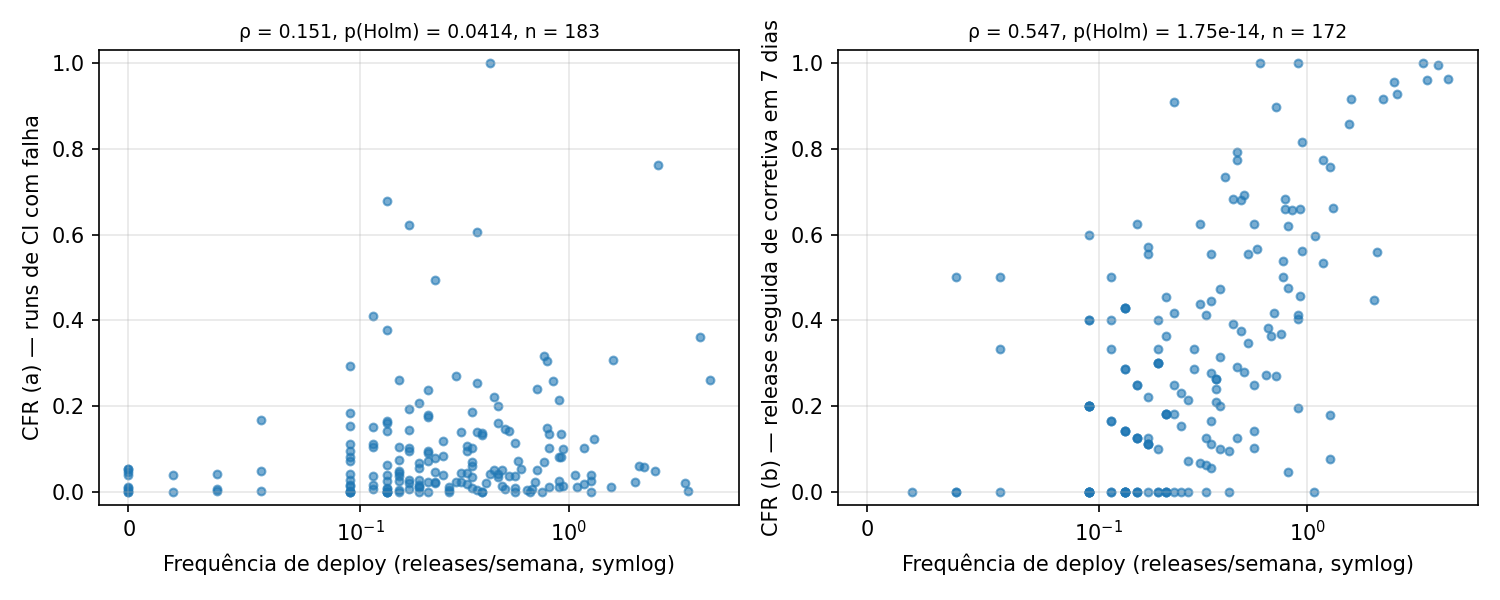
\includegraphics[width=\textwidth]{rq05/rq05_dispersao.png}
\caption{RQ05: frequência de deploy (eixo X em escala \textit{symlog}, que
mantém os 9 repositórios sem release na janela) versus CFR (a) e CFR (b).}
\label{fig:rq05}
\end{figure}

Nenhuma das variantes sustenta a afirmação do DORA de que velocidade e
estabilidade não competem, o que exigiria $\rho$ negativo. A magnitude no CFR
(b) é em parte induzida pela definição: com mais releases por semana, é mais
provável que uma release \textit{patch} ocorra nos sete dias seguintes e seja
marcada como corretiva. O CFR (a), que mede falha de pipeline e independe do
ritmo de releases, mostra associação fraca. Em ambos os casos trata-se de
associação monotônica, sem implicação causal: tamanho e atividade do projeto,
por exemplo, podem elevar as duas métricas. A validação parcial da heurística
(Seção~\ref{sec:validacao-cfrb}) indica ainda que o CFR (b) superestima as
releases corretivas, o que reforça a cautela com essa associação.

\subsection{RQ06: características dos repositórios}

Os fatores pré-registrados são linguagem principal (TypeScript 77, Python 60,
``Outras'' 51, que reúne as 16 linguagens com menos de 10 repositórios, Go 31,
JavaScript 31, Rust 25, C++ 13 e Java 10), quartis de estrelas (75 por quartil)
e quartis de contribuidores (74 a 76 por quartil). Dois repositórios não têm
linguagem principal. As métricas são as da configuração de referência C1. A
Tabela~\ref{tab:rq06} resume os 12 testes de Kruskal-Wallis, com tamanho de
efeito $\varepsilon^2 = H/(n-1)$.

\begin{table}[ht]
\centering
\caption{RQ06: Kruskal-Wallis por fator e métrica (C1). Células: $\varepsilon^2$
($p_{Holm}$); * indica significância após Holm. Fonte:
\texttt{analysis/rq06/rq06\_resultados.json} (\texttt{lab03.analysis.rq06}).}
\label{tab:rq06}
\small
\begin{tabular}{lcccc}
\hline
Fator & Frequência & Lead time (a) & CFR (a) & Recuperação \
 & $n = 300$ & $n = 289$ & $n = 300$ & $n = 268$ \
\hline
Linguagem ($k = 8$) & 0,055 (0,22) & 0,099 (0,002)* & 0,041 (0,82) & 0,027 (1,00) \
Estrelas ($k = 4$) & 0,010 (1,00) & 0,002 (1,00) & 0,022 (0,82) & 0,011 (1,00) \
Contribuidores ($k = 4$) & 0,007 (1,00) & 0,053 (0,017)* & 0,001 (1,00) & 0,017 (1,00) \
\hline
\end{tabular}
\end{table}

Dois dos 12 testes são significativos após a correção de Holm, ambos sobre o
lead time (a). Por linguagem, $H = 28{,}37$ ($p_{Holm} = 0{,}002$;
$\varepsilon^2 = 0{,}099$, médio): as medianas vão de 163~h em TypeScript e
181~h em Python a 565~h em Rust e 1.070~h em C++ (12 repositórios). Por quartil
de contribuidores, $H = 15{,}35$ ($p_{Holm} = 0{,}017$; $\varepsilon^2 =
0{,}053$, pequeno): a mediana é de 142~h e 157~h nos dois primeiros quartis e de
416~h e 403~h nos dois últimos, o que sugere entregas mais espaçadas em projetos
com mais colaboradores. Frequência, CFR (a), recuperação e estrelas não
diferem de forma significativa, e os efeitos nessas combinações são
desprezíveis ou pequenos ($\varepsilon^2 \le 0{,}055$). Os testes não indicam
quais grupos diferem entre si, pois não houve comparações \textit{post hoc}.
Linguagem e número de contribuidores podem refletir o tipo de projeto (por
exemplo, bibliotecas de sistemas contra aplicações web), que não foi
controlado. Como alguns grupos têm 10 a 13 repositórios, os resultados por
linguagem são menos estáveis. Medianas e IQR por grupo estão em
\texttt{analysis/rq06/rq06\_grupos.csv}. O tipo de projeto não foi usado como
fator, porque só está rotulado para os 60 repositórios da amostra-ouro.

\subsection{Validação do CFR (b): avaliador único}
\label{sec:validacao-cfrb}

O protocolo previa três avaliadores independentes e consenso sobre 300
releases. Isso não foi cumprido: por decisão do grupo, a segunda rodada
(\texttt{labels/reamostragem-v2/}) não foi rotulada, e na primeira rodada só um
integrante (avaliador B) rotulou as releases. Os rótulos do avaliador A são
rascunhos gerados por IA, marcados como tal em todas as linhas. Por isso não
há consenso nem medida de confiabilidade entre avaliadores. O resultado a
seguir é uma \emph{validação de avaliador único} e não o F1 contra consenso
previsto no protocolo.

A primeira rodada foi sorteada da mesma coleta do snapshot (13 de outubro de
2026, mesma janela). Com o dataset de 300 repositórios, todas as 283 releases
sorteadas, em 58 repositórios, constam do snapshot e têm identificador e
veredito da heurística conferidos, e nenhuma foi excluída. A
Tabela~\ref{tab:validacao-cfrb} compara a heurística v2 com os rótulos de B.

\begin{table}[ht]
\centering
\caption{CFR (b): heurística v2 × avaliador B (283 releases, 58 repositórios).
IC 95\% de Wilson. Fonte: \texttt{analysis/validacao\_cfr\_b/resultados.json}
(\texttt{lab03.analysis.cfr\_b\_validation}).}
\label{tab:validacao-cfrb}
\small
\begin{tabular}{lrr|lr}
\hline
B $\backslash$ heurística & não & sim & Métrica & Valor [IC 95\%] \\
\hline
não & 109 & 128 & Precisão & 0,238 [0,180--0,308] \\
sim & 6 & 40 & Recall & 0,870 [0,743--0,939] \\
 & & & F1 & 0,374 \\
\hline
\end{tabular}
\end{table}

A heurística deixa escapar poucas releases corretivas (6 de 46), mas só 40
das 168 releases que ela marca como corretivas foram confirmadas por B. O F1
fica bem abaixo do limiar de 0,70 do protocolo. O CFR (b) deve, portanto, ser
lido como tendendo a superestimar a taxa de falha. Uma explicação plausível,
ainda não verificada caso a caso, são as releases \textit{patch} publicadas em
até sete dias sem corrigir a entrega anterior.
Como referência auxiliar, e não como segundo avaliador, os rascunhos de IA
concordam com B em 88\% das releases ($\kappa$ de Cohen $= 0{,}590$). Os
intervalos tratam as releases como independentes, embora venham agrupadas em
cinco por repositório, e por isso são otimistas. Com um único avaliador, erros
ou critérios pessoais de B não podem ser separados do erro da heurística.

\subsection{RQ07: sensibilidade da classificação}

Comparando a categoria geral entre as variantes, há mudança em todos os pares
(Tabela~\ref{tab:rq07}). Só entram repositórios classificados nas duas
variantes; os demais são excluídos, sem imputação. O kappa de Cohen usa pesos
lineares para a ordem Low $<$ Medium $<$ High $<$ Elite.

\begin{table}[ht]
\centering
\caption{RQ07: mudanças de categoria geral e concordância entre variantes
(300 repositórios). Fonte: \texttt{analysis/rq07/rq07\_resultados.md}
(\texttt{lab03.analysis.rq07}).}
\label{tab:rq07}
\small
\begin{tabular}{lrrrrrr}
\hline
Par & $n$ & Excluídos & Mudaram (\%) & Subiram & Desceram & $\kappa$ linear \\
\hline
C1$\times$C2 & 259 & 41 & 115 (44,4\%) & 36 & 79 & 0,311 \\
C1$\times$C3 & 260 & 40 & 74 (28,5\%) & 59 & 15 & 0,625 \\
C2$\times$C3 & 261 & 39 & 107 (41,0\%) & 99 & 8 & 0,428 \\
\hline
\end{tabular}
\end{table}

Nas exclusões, 38 repositórios não têm categoria em nenhuma variante em cada
par; além deles, C1$\times$C2 exclui 2 sem C1 e 1 sem C2, C1$\times$C3 exclui
4 sem C1, e C2$\times$C3 exclui 3 sem C2. A C3 não tem exclusões isoladas.
As mudanças que envolvem C2 exigem cautela: ela usa o CFR (b), cuja validação
de avaliador único obteve F1 = 0,374, abaixo do limiar de 0,70. Portanto, parte
das diferenças pode refletir erro da heurística, não apenas a definição de
entrega. Os resultados descrevem esta amostra e não implicam causalidade.
